\subsection{RQ3: Do the coverage metrics transfer between AV implementation?}

In this paper, we presented a framework for improving the predicate coverage for test scenarios for AVs.
% 
One of the drawbacks of our proposed method is that it requires the AV to be deployed in-the-loop.
% 
Since different AV implementations react to the same scenario in different ways, the coverage metrics for the same collection of test scenarios can vary based on the AV implementation.
% 
This begs the question, do test cases that improve coverage for one AV implementation also work for other implementations?
% 
Such transfer of coverage would be immensely helpful as it points out to the common set of use-cases or corner cases among different implementations.

To answer this question, we investigate the transfer of coverage metrics from one implementation to the other.
% 
That is, we collect all the test scenarios generated by the fuzzer of choice for a given AV implementation.
% 
We then subject other AV implementations to the same set of test scenarios and measure the coverage.
% 
We normalize the coverage of the current AV implementation as $100\%$ and plot the predicate coverage of the transferred AV implementation as a percentage.
% 
For example, we collect all the test scenarios generated by Atheris on CARLA Autopilot and deploy the same scenarios on CARLA BehaviorAgent, TF++, and SCENIC agent.
% 
We plot the coverage of each of the three individual agents relative to the original coverage.
% 
We use only two fuzzing methods, first is the code coverage based Atheris and second is the PCGF-AFLFast fuzzer. 
%
We perform 10 trials using $\{ 0, \dots, 9 \}$ PRNG seeds as in RQ1-2 where each trial consists of generating a corpus using a fuzzer and an ego agent, then testing the corpus on a different ego agent.
%
The PRNG seed is fixed between the generation and test experiments.
%
% For each pair different agents, we consider 10 trials using the 

% In this part, we evaluate whether fuzzing can generate high-coverage driving scenarios irrespective of AV implementation.
% 


%---------------------
% \subsubsection{Performance Metric}
% Ratio of coverage sizes, where the target coverage is when the original ego agent is used to generate the test-cases, and the test coverage is when the different test ego agents are tested on the test-suite
% 
% 
% \subsubsection{Fuzzer}
% We use PCGF-AFLFast for this part, since it was the best performing fuzzer, also that the experiments for the other fuzzers did not finish in time for the submission deadline.


%---------------------
% \subsubsection{Trials}


\begin{figure}
    \centering
    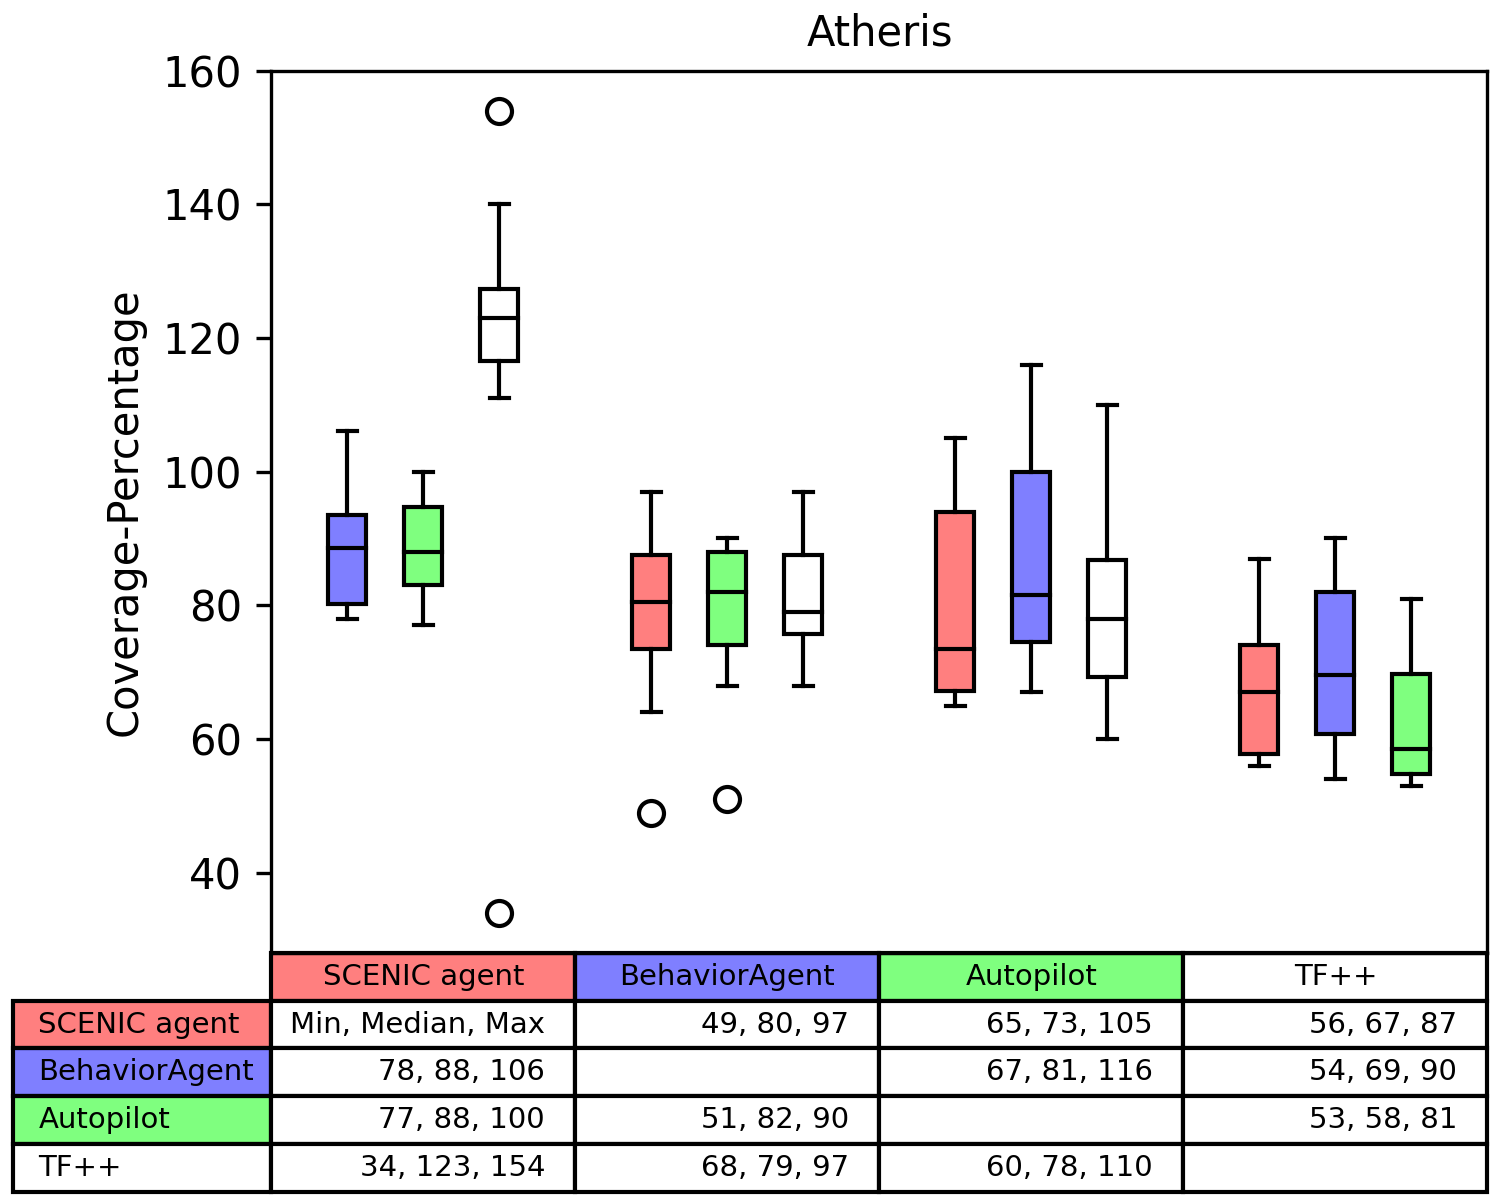
\includegraphics[width=0.7\linewidth]{figures/chapter5/RQ3/Atheris_traffic-rules_all-coverage_PredicateSetCoverage_Coverage-Percentage.png}
    \caption{Common set of scenarios for different agents}
    \label{fig:switch-agent_Atheris}
\end{figure}

\begin{figure}
    \centering
    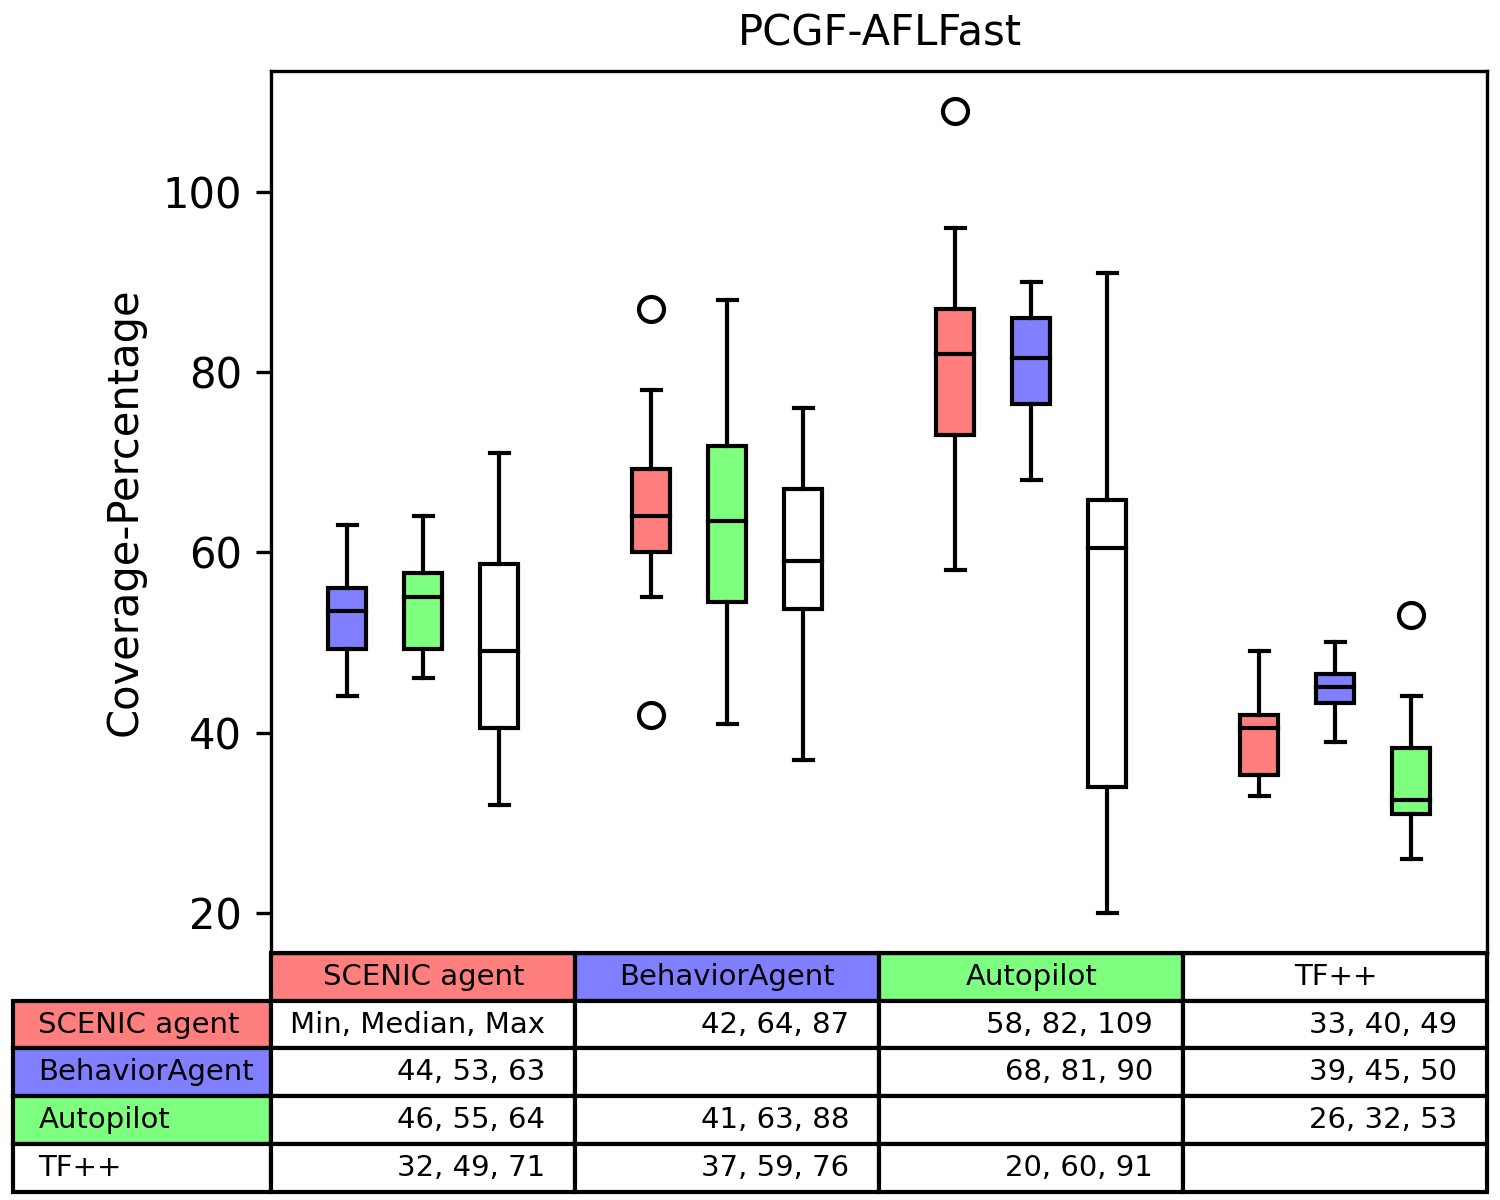
\includegraphics[width=0.7\linewidth]{figures/chapter5/RQ3/PCGF_traffic-rules_all-coverage_PredicateSetCoverage_Coverage-Percentage.png}
    \caption{Common set of scenarios for different agents}
    \label{fig:switch-agent_Random}
\end{figure}

%---------------------
\subsubsection{Results}
The transfer of coverage metrics from one AV implementation to another are presented in Figure~\ref{fig:switch-agent_Atheris} and Figure~\ref{fig:switch-agent_Random}.
% 
Each column of the table shows the agent used to generate the corpus, and each row shows the agent tested on the resulting corpus.
%
The entries of the table show the minimum, median, and maximum of the metric accross the 10 trials.
%
Above the table, we show the standard box-plot of the results, i.e. quartiles, median, and fliers.


The first observation is that scenarios generated for one agent are indeed reusable for other agents.
%
For code driven fuzzing tool Atheris, on average, one can obtain $70\%$ of the original coverage by applying the same set of test cases to a different implementation; this number drops close to $50\%$ for PCGF-AFLFast.
% 
% \textbf{Insert a line here for PCGF-AFLFast and compare if it is higher or lesser}.
%
% 
% 
Another observation is that transfer of coverage is better between Autopilot, SCENIC agent, and BehaviorAgent as opposed to TF++.
% 
One possible reason is that all these three agents do not implement perception processing and the maps and relative positions of other vehicles is provided to these agents by the CARLA environment.
% 
This also explains why the coverage metrics from TF++ transferred poorly to other agents because TF++ learns the road network and the position of other agents through perception.
% 
The authors would like to confirm this hypothesis by conducting more experiments on open source end-to-end CARLA Leaderboard agents; however, much to our chagrin, we couldn't find one.
% 

The second observation is that the scenarios generated using PCFG-AFLFast transfer poorly when compared to Atheris for almost all instances.
% 
This highlights that while PCGF-AFLFast increases scenario coverage, it improves the coverage for a specific AV implementation.
% 
From the results of RQ1, we remarked that PCGF is fast enough to generate more number of test scenarios and accurate enough to improve coverage; however, this evaluation highlights that the coverage is implementation specific.

The third observation is that in some instances the predicate coverage transfer is more than $100\%$. 
% 
While this may be counterintuitive, it deserves some explanation.
% 
Consider a test-suite $\{ s_1, s_2 \}$ for a given AV implementation, say CARLA Autopilot.
% 
If we subject a different AV implementation, say TF++, to these two scenarios $s_1$ and $s_2$, TF++ might react in different ways than Autopilot; causing an increase in the predicate coverage.



